
\chapter{Análisis Teórico de la Aplicación del Internet de las Cosas en los Museos} \label{cap:analisis_teorico}

\addcontentsline{toc}{section}{Introducción}
        \textbf{\Large Introducción}\newline

        En este capítulo se analiza el estado del arte del Internet de las Cosas y su aplicación en los museos a nivel internacional y nacional, así como la caracterización de la
        Colección de Arte y Arqueología Francisco Prat Puig teniendo en cuenta su estado en cuanto a la conservación de las piezas allí presentes. También se abordan las arquitecturas propuestas para IoT y la estipulación de una para el presente proyecto analizándola por partes.
        Además se hace el análisis de las condiciones que favorecen el ataque de insectos xilófagos en las estructuras y en las obras pertenecientes a la colección, así como los daños ocasionados por la variación de los valores de las variables microclimáticas tomando como referencias los recomendados por los autores.

    \section{Internet de las Cosas}\label{sec:iot}

    El Internet de las Cosas describe objetos físicos (o grupos de estos) con sensores, capacidad de procesamiento, software y otras tecnologías que se conectan e intercambian datos con otros dispositivos y sistemas a través de internet u otras redes de comunicación.

    Este campo ha evolucionado gracias a la convergencia de múltiples tecnologías, como la informática ubicua, los sensores, los sistemas integrados cada vez más potentes y el aprendizaje automático \cite{carrasco}. 

    Los campos tradicionales de los sistemas embebidos, las redes de sensores inalámbricos, los sistemas de control y la automatización (incluida la domótica y la inmótica) hacen posible, de forma independiente y colectiva, el Internet de las cosas \cite{lennox}.

    El IoT como arquitectura emergente basada en la Internet global presta la posibilidad de intercambio de bienes y servicios entre redes de la cadena de suministro y que tiene un impacto importante en la seguridad y privacidad de los actores involucrados \cite{weber}. 

    \subsection{IoT en los museos internacionales}\label{sec:iotMundo}
        
        En el grupo de las bibliografías consultadas existen diversos ejemplos del empleo del IoT en los museos.

        En el caso del Conjunto Monumental de San Domenico Maggiore, ubicado en Nápoles (Italia), dentro del mismo se han transformado más de 270 esculturas en obras de arte parlantes. Equipado con un tablero de sensores, cada objeto puede proponerse automáticamente a los visitantes, compartiendo su historia en diferentes modalidades e idiomas, lo que permite un proceso de disfrute novedoso durante una experiencia cultural. \cite{monumentoSanDomenico}.
    
        En la Universidad de El Cairo, Egipto, desarrollaron un sistema para la conservación de las piezas en los museos, un sistema que no solo mide los atributos del entorno, sino que también mantiene la seguridad de los artefactos al detectar cualquier prueba de contacto o movimiento. También controla la intensidad de la luz en función de la ocupación de la sección del museo. Una característica diferenciadora del sistema es el diseño de energía ultrabaja de su nodo sensor que conduce a una larga vida útil de hasta 50 días. \cite{ultraLowPowerConservacion}.
    
        Estos son solo dos de los ejemplos. La tabla \ref{tab:iot_internacional} muestra una relación de otros autores que emplean el IoT en los museos. Pero antes, para poder comprender la tabla \ref{tab:iot_internacional} se define una primera tabla en la que se le otorga a cada autor un número de manera tal que se entienda quien es cada autor. Por lo que se define la tabla \ref{tab:numeracion_autores}:

    \begin{table}[H]
        \centering
        \caption{Numeración autores}
        \begin{tabular}{|c|c|}
        \hline
        \rowcolor[HTML]{9698ED} 
        Autor & Numeración Asociada \\ \hline
        Maksimovic y Cosovic \cite{maksimovic}     & 1                   \\ \hline
        Shah y Mishra \cite{shan}     & 2                                \\ \hline
        Marshall \cite{marshall}     & 3                                 \\ \hline
        Ghosh, Roy, y Saha \cite{ghosh}     & 4                          \\ \hline
        Rao, Sharma, y Narayan \cite{rao}     & 5                        \\ \hline
        Alletto y cols. \cite{alletto}     & 6                           \\ \hline
        Alsuhly y Khattab \cite{alsuhly}     & 7                         \\ \hline
        Spachos y Plataniotis \cite{spachos}     & 8                     \\ \hline
        Lopez-Martínez, Iglesias, y Carrera \cite{lopezmartinez}     & 9\\ \hline
        \end{tabular}
        \label{tab:numeracion_autores}
    \end{table}

    \begin{table}[h]
        \centering
        \caption{IoT en los museos internacionales}
        \begin{tabular}{|c|l|l|}
        \hline
        \rowcolor[HTML]{9698ED} 
        Manifestación       & Mediciones                                                                                                                                                        & Tecnología                                                                                                                                              \\ \hline
        Temperatura         & {(}1,2,7{)} Temperatura °C                                                                                                                                        & \begin{tabular}[c]{@{}l@{}}{(}1{)} RPI, Sensores, Cloud\\ SVM (Árboles de Decisiones),\\ {(}2{)} IoT-WSMP,\\ {(}7{)} RPI, ESP32, Node-Red.\end{tabular} \\ \hline
        Humedad             & {(}1,2,7{)} Humedad \%                                                                                                                                            & \begin{tabular}[c]{@{}l@{}}{(}1{)} RPI, Sensores, Cloud\\ SVM (Árboles de Decisiones),\\ {(}2{)} IoT-WSMP,\\ {(}7{)} RPI, ESP32, Node-Red.\end{tabular} \\ \hline
        Intensidad luminosa & {(}2,7{)} Lumens                                                                                                                                                  & \begin{tabular}[c]{@{}l@{}}{(}2{)} IoT-WSMP,\\ {(}7{)} RPI, ESP32, Sensores.\end{tabular}                                                               \\ \hline
        Vibraciones         & {(}1{)} Estabilidad del Edificio (Hz)                                                                                                                             & \begin{tabular}[c]{@{}l@{}}{(}1{)} RPI, Sensores, Cloud\\ SVM (Árboles de Decisiones).\end{tabular}                                                     \\ \hline
        Humo                & {(}1{)} C02 ppm                                                                                                                                                   & \begin{tabular}[c]{@{}l@{}}{(}1{)} RPI, Sensores, Cloud\\ SVM (Árboles de Decisiones).\end{tabular}                                                     \\ \hline
        Polución            & {(}1{)} Polvo                                                                                                                                                     & \begin{tabular}[c]{@{}l@{}}{(}1{)} RPI, Sensores, Cloud\\ SVM (Árboles de Decisiones).\end{tabular}                                                     \\ \hline
        Xilófagos           & {(}1{)} Plagas de madera                                                                                                                                          & \begin{tabular}[c]{@{}l@{}}{(}1{)} RPI, Sensores, Cloud\\ SVM (Árboles de Decisiones).\end{tabular}                                                     \\ \hline
        Personas            & \begin{tabular}[c]{@{}l@{}}{(}7{)} Aceleración, Toque.\\ {(}8{)} Geolocalización.\\ {(}3{)} Movimiento\\ {(}9{)} Propuestas de juegos\\en el museo\end{tabular}  & \begin{tabular}[c]{@{}l@{}}{(}1{)} PIR, {(}4{)} IA,\\ {(}5{)} RPI, ESP32, Sensores.\end{tabular}                                                        \\ \hline
        \end{tabular}
        \label{tab:iot_internacional}
    \end{table}

    \vspace{1.5cm}

    Como se puede observar en la tabla \ref{tab:iot_internacional} el mayor número de autores analizados centran su atención en el usuario que accede al museo en aras de brindarle una propuesta agradable en su visita.

    \subsection{Internet de las Cosas en Cuba}\label{sec:iotCuba} 

    En el contexto cubano, hasta el momento solo se tiene referencia de un artículo científico publicado en Cuba por Mengana de la Fe \cite{lopezramos} en el Museo Emilio Bacardí de la Ciudad de Santiago de Cuba con el uso de la RA,
    sin integración con otras tecnologías, pero se demuestra el interés de insertar esta dentro del pueblo cubano ya que hay referencias de proyectos enfocados a la educación y a los videojuegos en noticias o eventos organizados por instituciones cubanas.
    Por su parte el uso del IoT se evidencia en el turismo tal como lo analiza Franco \cite{franco} y Cordova y cols. \cite{cordovacorso}, en la protección del medio ambiente de Morales \cite{morales} y para el control de acceso de personal no autorizado por parte de Cruz y cols. \cite{cruzrojas}.

    Otros de los ejemplos de la aplicación del IoT en nuestro país lo constituyen el sistema IoT para el control del nivel de tanques de agua de La Habana \cite{herrera2020}, en el cual se brinda una solución desarrollada sobre Arduinos utilizando transporte de telemetría de mensajes en cola (MQTT, Message Queing Telemetry Transport)
    como protocolo de comunicación máquina-máquina (M2M) a través de un servidor Mosquitto. Tal es el caso también de la alternativa \textit{Open Source} en la implementación de un sistema IoT para la medición de la calidad del aire con el empleo de tarjetas de desarrollo Arduino, ESP8266 y de sensores destinados a la captura de la concentración de CO2 y gases generales, así como densidad de polvo \cite{ochoa2018alternativa}.
    
    Aun cuando existan más ejemplos del empleo del Internet de las Cosas en Cuba, no se ha encontrado evidencia de su aplicación en los museos cubanos, de ahí el aporte novedoso de este proyecto.

    \section{Colección de Arte y Arqueología Francisco Prat Puig}\label{sec:coleccion_prat}

    Como parte de las entrevistas con los especialistas y los recoridos en la colección se identificaron aspectos a destacar tales como:

    \begin{itemize}
        \item Presenta daños causados por la incidencia de las variables ambientales o ataques biológicos de xilófagos en los bienes patrimoniales que se encuentran en exposicion o en el almacen. Principalmente para aquellos confeccionados con materiales como son: el papel, cuero, tela y madera.
        \item Imposibilidad de conocer o controlar el estado de conservación de los elementos patrimoniales en tiempo real.
        \item No existe ningún tipo de tecnología implementada en la colección para los especialistas ni hacia el público visitante.
        \item Insuficiente control ambiental, seguridad y prevención de posibles daños en el futuro de la colección.
    \end{itemize}

    En síntesis, se puede afimar que la gestión de la colección de Artes y Arqueología Francisco Prat Puig carece de una intervención tecnológica que favorezca la calidad en la toma de decisiones para su conversacion preventiva.\\

    La colección Francisco Prat Puig está distribuida de tal modo que las piezas están ubicadas en tres salas. Enumerándolas: sala 1, sala 2 y sala 3.\\
    La sala 1 (figura \ref{imag:sala_1}) está caracterizada por la presencia de varios objetos distribuidos en vitrinas, sobre mesas, colgados, en estantes empotrados en la pared, o en pedestales. Se observan piezas de cerámica, marfil, metal, piedra, madera, entre otros materiales, así como colecciones de numismática.\newline
    
    \begin{figure}[H]
        \centering
        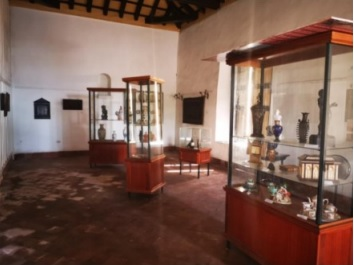
\includegraphics[width=8cm, height=6cm]{imagenes/sala_1.jpg}
        \caption{Exposición permanente}
        \label{imag:sala_1}
    \end{figure}

    \newpage

    En la sala 2 solamente se encuentran pinturas pertenecientes a la colección, estas poseen también condiciones de deterioro notables por el efecto de la humedad y del nivel de luz dentro del local.

    % [Imagen de la sala 2]\newline
    Dentro de la sala 3 (figura \ref{imag:sala_3}) se localizan también varios objetos ubicados en pedestales mostrando colecciones de medallas y objetos personales del mismo Prat Puig y, además, vitrinas donde se hallan, principalmente, objetos de cerámica como platos, jarrones y cántaros.\newline
    
    \begin{figure}[H]
        \centering
        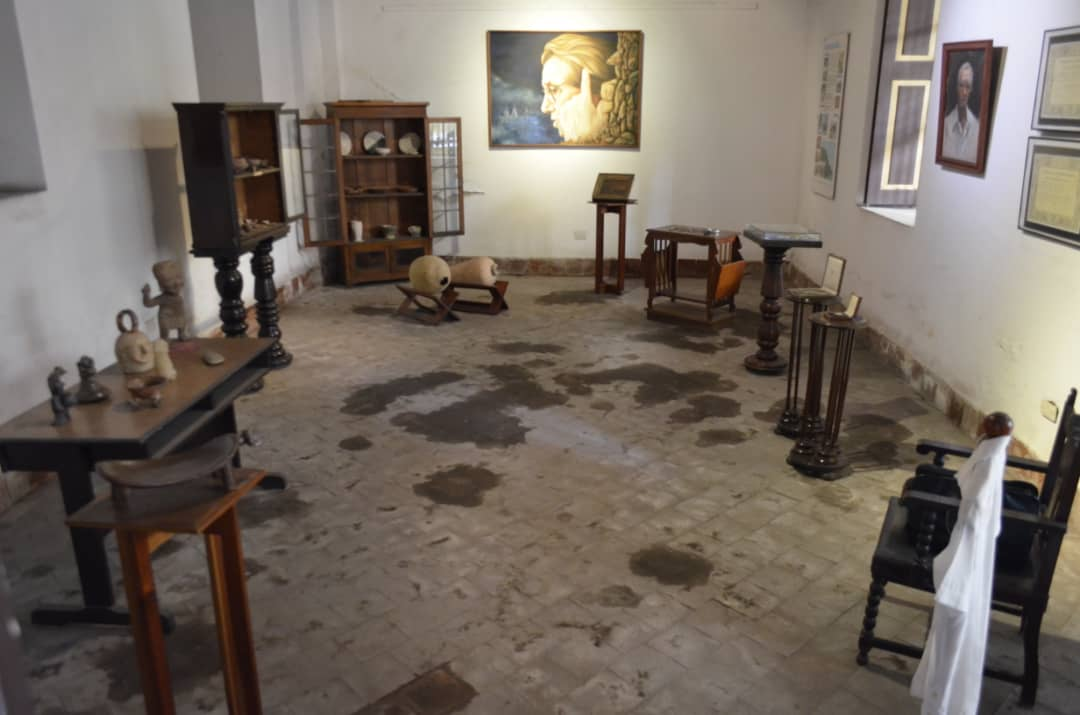
\includegraphics[width=8cm, height=6cm]{imagenes/sala_3.jpeg}
        \caption{Sala Memorial}
        \label{imag:sala_3}
    \end{figure}

    En el gráfico que se muestra a continuación se relaciona el valor cuantitativo de las principales formas en las que se exponen las piezas dentro de estas salas pertenecientes a la colección.

    \begin{figure}[H]
        \centering
        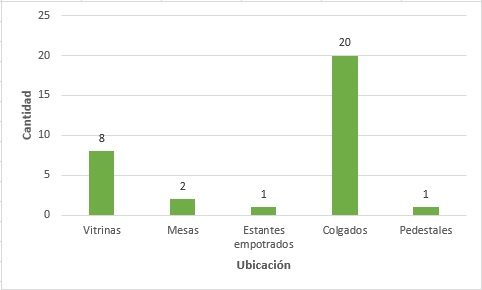
\includegraphics[width=10cm, height=6cm]{imagenes/formas expositivas.jpg}
        \caption{Ubicación piezas}
        \subcaption*{Fuente: Elaboración propia}
        \label{imag:ubicacion_piezas}
    \end{figure}

    Según la figura \ref{imag:ubicacion_piezas}, varios objetos están dispuestos dentro de vitrinas donde, al encontrarse protegido por paredes de cristal, se genera un microclima\footnote{microclima: según el diccionario Oxford, es el conjunto de las condiciones climáticas particulares de un lugar determinado, resultado de una modificación más o menos acusada y puntual del clima de la zona en que se encuentra influido por diferentes factores ecológicos y medioambientales.}, por lo que la condición ambiental en estas es diferente a la condición ambiental de la sala, de ahí la necesidad de incorporar nodos de tal manera que se tomen los datos dentro de estas vitrinas y, además, un nodo para la sala en general.

    \section{Arquitectura IoT y sus principales capas}\label{sec:arquitecturas}

    No existe una única definición universalmente adoptada, estándar, de Arquitectura de IoT; diferentes propuestas han surgido durante su desarrollo. Se abarcan tecnologías de comunicación, dispositivos de cómputo, sensores y actuadores \cite{ioT_en_Cosas_de_salud}.
    
    La arquitectura de IoT es principalmente desarrollada por capas, dígase, la arquitectura de 3 capas, la arquitectura de 5 capas, la arquitectura de Nube, la arquitectura de niebla y la arquitectura de computación de Borde, solo por mencionar algunas \cite{arquitecturaIEEE}.\\

    \begin{figure}[H]
        \centering
        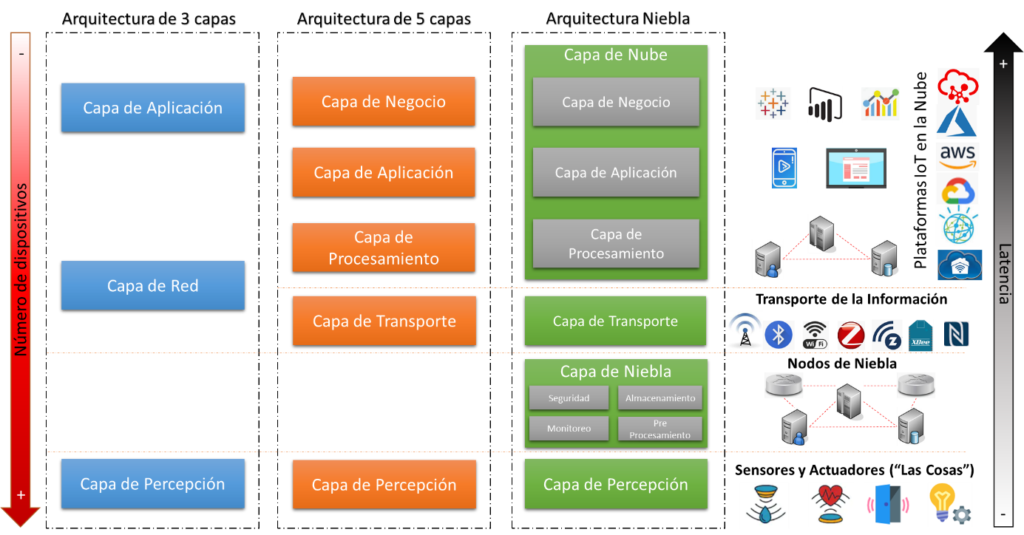
\includegraphics[width=8cm, height=5cm]{imagenes/Comparacion-arquitecturas-1024x535}
        \caption{Comparación arquitecturas}
            \subcaption*{Fuente: García \cite{arquitecturaPaginaLuisGarcia}}
        \label{imag:comparacionArquitecturas}
    \end{figure}

    En la figura \ref{imag:comparacionArquitecturas} se desarrolla una comparación entre las arquitecturas de 3 capas, 5 capas y la arquitectura niebla.

    \newpage

    Según Ciberseguridad \cite{capasIoTciberseguridad}, la mayoría de estas arquitecturas de IoT se basan en fundamentos básicos:
    \begin{itemize}
        \item Dispositivos más inteligentes en una forma diferente.
        \item Red y puerta de enlace que permite que los dispositivos formen parte del IoT.
        \item Middleware que incluye espacios de almacenamiento de datos y avances en las capacidades de predicción.
        \item Aplicaciones de usuario final.
    \end{itemize}

    Existen varias arquitecturas, marcos de referencia o modelos conceptuales para IoT propuestos por organizaciones, comunidad académica y el sector empresarial. Las propuestas de arquitecturas pueden variar de autor en autor, en dependencia de la estructura del sistema IoT propuesto. Dichas arquitecturas son desarrolladas por capas en las que se agrupan los objetos, dispositivos, sensores, actuadores, entre otros. \cite{internetOfThingsStateOfTheArt} \cite{capasIoTciberseguridad}.\\

    En la figura \ref{imag:modelos_arquitecturas_iot} se representa una comparativa de algunos modelos basados en capas. Para propiciar una mejor comprensión de la figura \ref{imag:modelos_arquitecturas_iot} se desarrolló la tabla \ref{tab: referencias_capas} donde se muestra la relación de los autores referidos a las capas del IoT.

    \begin{table}[H]
        \centering
        \caption{Referencias figura \ref{imag:modelos_arquitecturas_iot}}
        \begin{tabular}{|l|l|}
        \hline
        \textbf{No. de Capas}    & \textbf{Referencias}                                                                                                                                              \\ \hline
        \multirow{2}{*}{3 capas} & \multirow{2}{*}{\begin{tabular}[c]{@{}l@{}}\cite{ref10} \cite{ref13} \cite{ref15}\\ \cite{ref16} \cite{ref19} \cite{ref25}\end{tabular}} \\
                                 &                                                                                                                                                                   \\ \hline
        4 capas                  & \begin{tabular}[c]{@{}l@{}}\cite{ref10} \cite{ref12} \cite{ref13}\\ \cite{ref19} \cite{ref16}\end{tabular}                          \\ \hline
        5 capas                  & \begin{tabular}[c]{@{}l@{}}\cite{ref9} \cite{ref10} \cite{ref13}\\ \cite{ref19} \cite{ref16}\end{tabular}                          \\ \hline
        Basado en SOA            & \begin{tabular}[c]{@{}l@{}}\cite{ref4} \cite{ref8} \cite{ref9}\\ \cite{ref15}\end{tabular}                                                        \\ \hline
        Basado en Middleware     & \cite{ref9}                                                                                                                                                \\ \hline
        6 capas                  & \cite{ref19}                                                                                                                                                        \\ \hline
        \end{tabular}
        \label{tab: referencias_capas}
    \end{table}

    \begin{figure}[H]
        \centering
        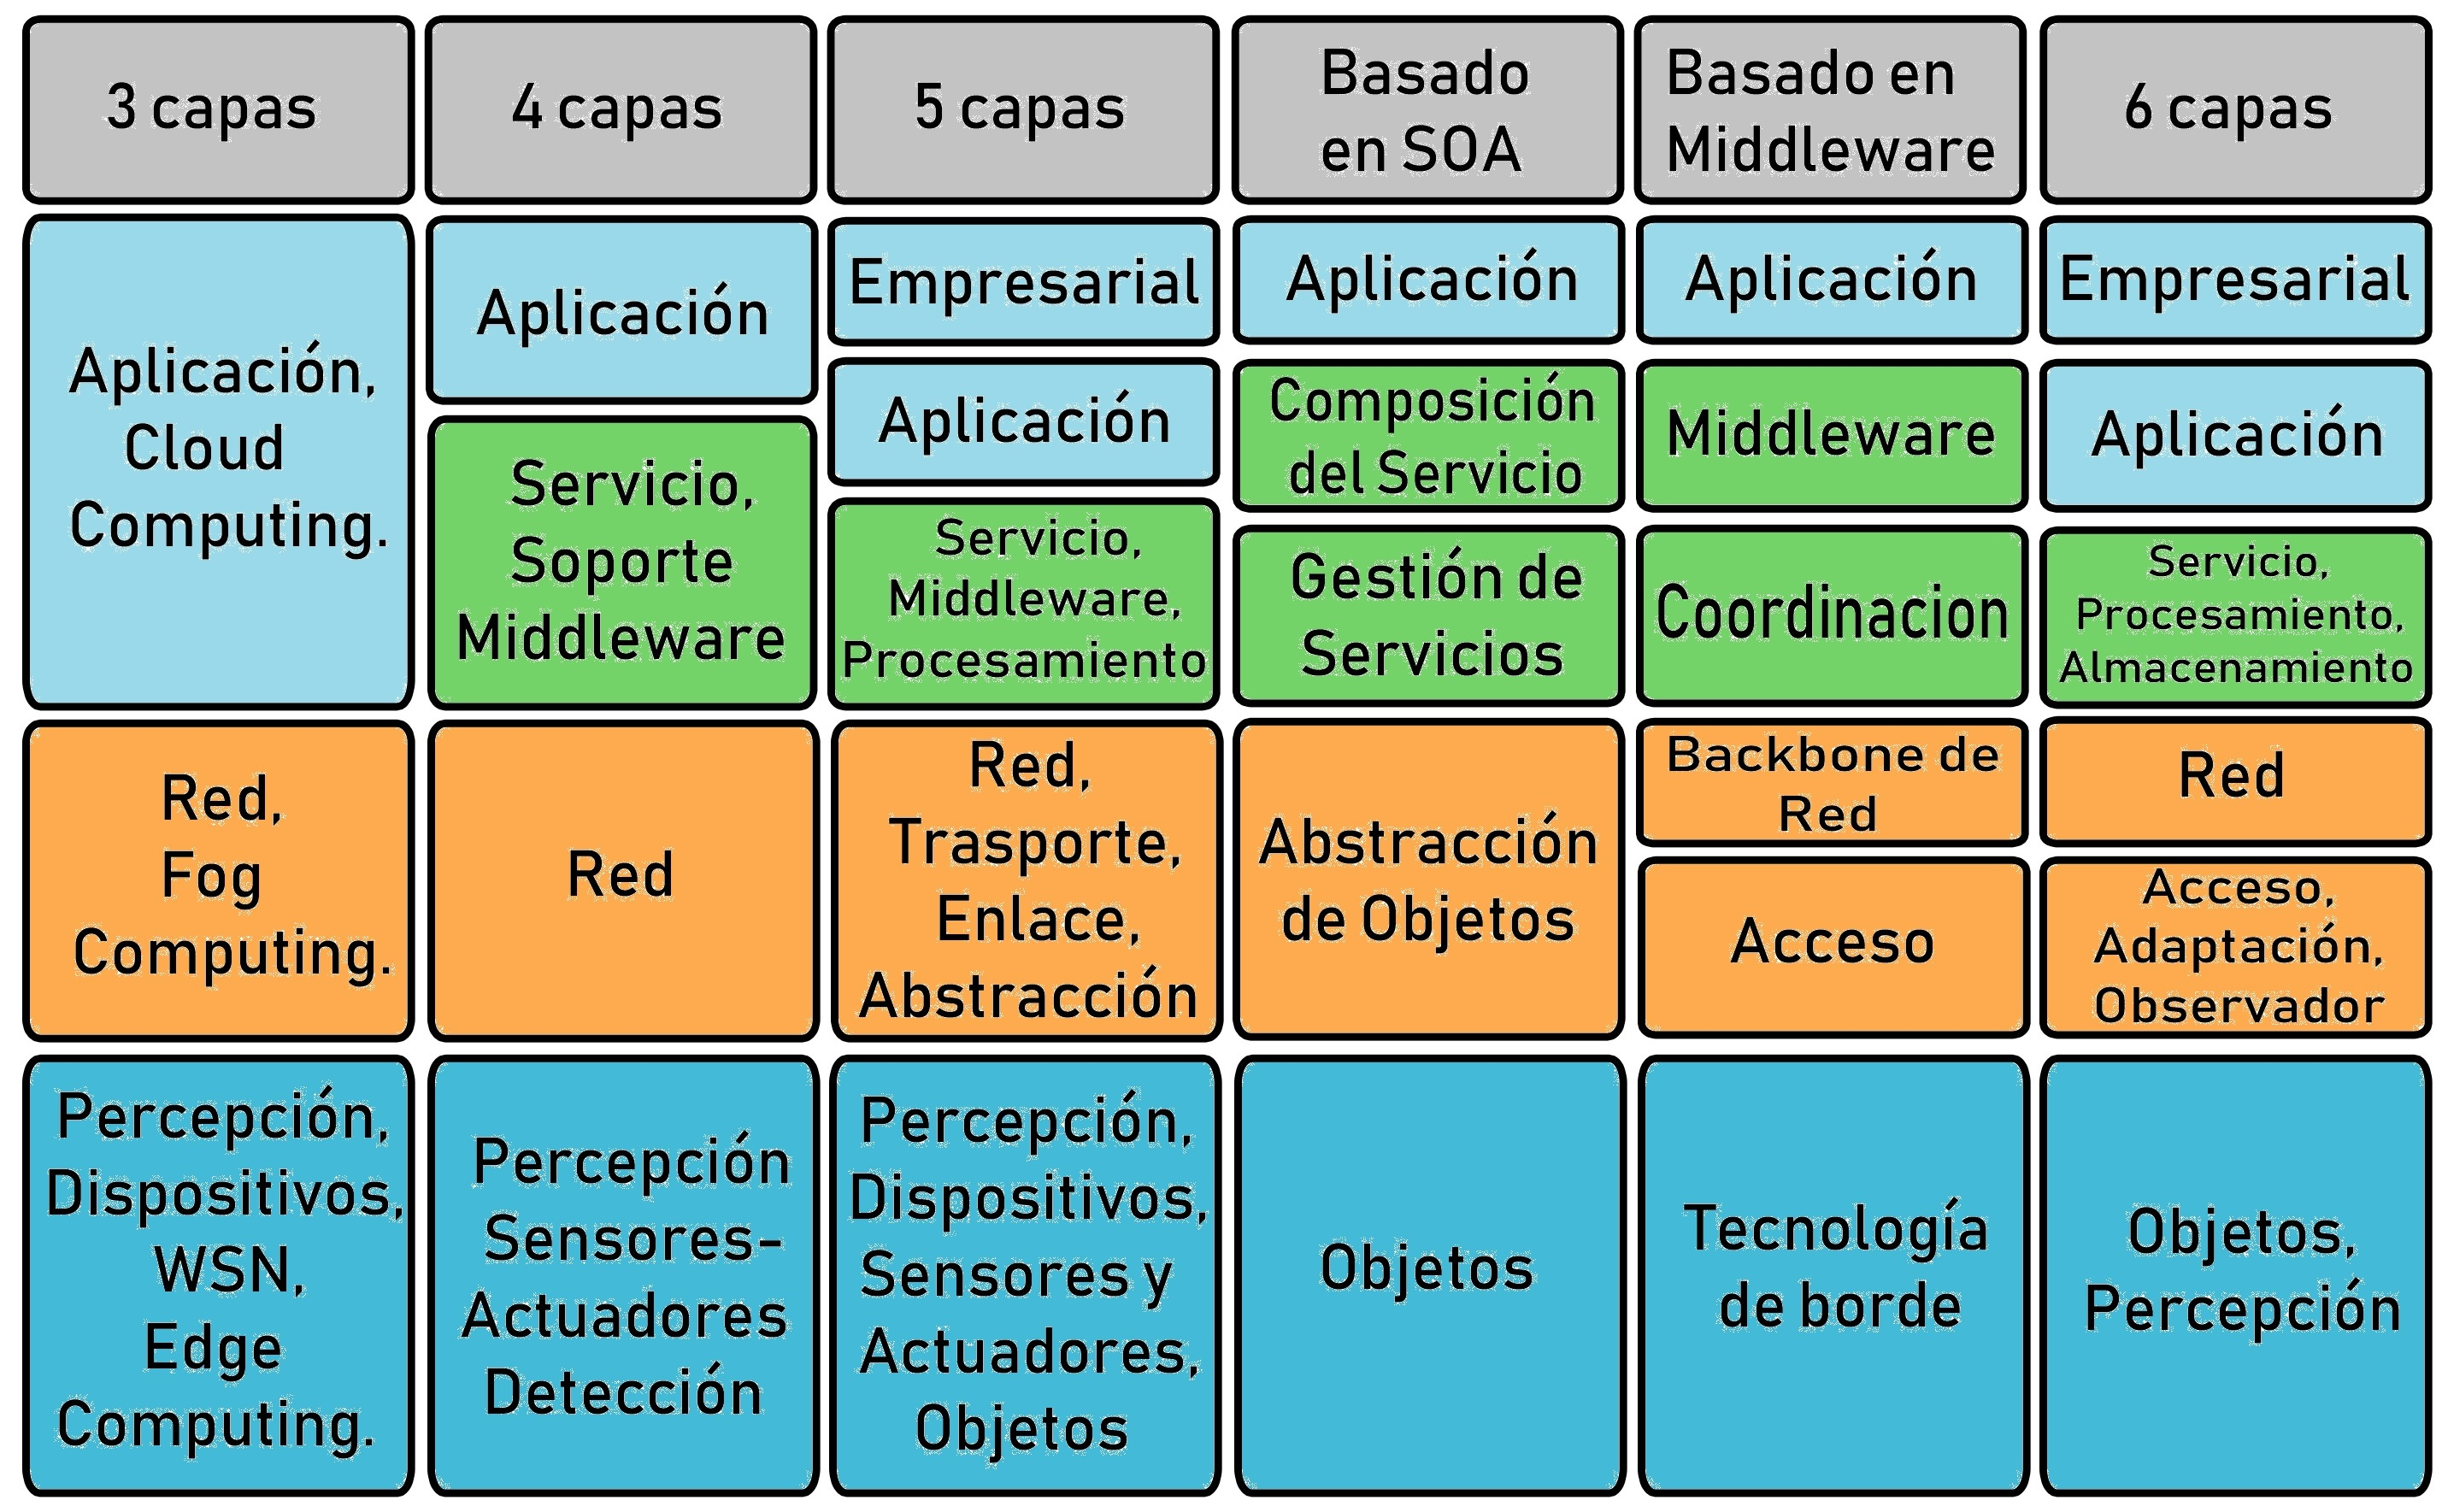
\includegraphics[width=15.6cm, height=9cm]{imagenes/capas.jpg}
        \caption{Modelos de arquitecturas IoT basados en capas}
        \subcaption*{Fuente: Elaboración propia}
        \label{imag:modelos_arquitecturas_iot}
    \end{figure}

    Desde el punto de vista de Ciberseguridad \cite{capasIoTciberseguridad} existen capas fundamentales dentro de la esctructura de IoT. En la tabla \ref{tab: capas_IoT} se detallan estas capas:

    \begin{table}[h]
        \centering
        \caption{Capas de IoT}
        \subcaption*{Fuente: \cite{capasIoTciberseguridad}}
        \begin{tabular}{|l|l|}
        \hline
        \rowcolor[HTML]{9698ED} 
        \textbf{Capas}                                                             & \textbf{Descripción}                                                                                                                                                         \\ \hline
                                                                                   &                                                                                                                                                                              \\
        \multirow{-2}{*}{Capa de percepción}                                       & \multirow{-2}{*}{Administra dispositivos inteligentes en todo el sistema.}                                                                                                   \\ \hline
        \begin{tabular}[c]{@{}l@{}}Capa de conectividad/\\ transporte\end{tabular} & \begin{tabular}[c]{@{}l@{}}Permite transferir datos desde la nube a los dispositivos\\ y viceversa, diferentes aspectos de las puertas de enlace\\ y las redes.\end{tabular} \\ \hline
        Capa de procesamiento                                                      & \begin{tabular}[c]{@{}l@{}}Controla y administra los niveles de IoT para optimizar\\ los datos en todo el sistema.\end{tabular}                                              \\ \hline
        Capa de aplicación                                                         & \begin{tabular}[c]{@{}l@{}}Ayuda en los procedimientos de análisis, control de\\ dispositivos e informes a los usuarios finales.\end{tabular}                                \\ \hline
        Capa empresarial                                                           & \begin{tabular}[c]{@{}l@{}}Deriva información y análisis de toma de decisiones\\ a partir de datos.\end{tabular}                                                             \\ \hline
        Capa de seguridad                                                          & \begin{tabular}[c]{@{}l@{}}Cubre todos los aspectos de protección de toda la\\ arquitectura de IoT.\end{tabular}                                                             \\ \hline
        Capa de borde                                                              & \begin{tabular}[c]{@{}l@{}}Funciona en un bode o cerca de la recopilación\\ de información del dispositivo.\end{tabular}                                                     \\ \hline
        \end{tabular}
        \label{tab: capas_IoT}
        \end{table}

    Por otra parte B. Mazon y A. Pan Olivo \cite{internetOfThingsStateOfTheArt} plantean que dentro de las capas más importantes del IoT podemos encontrar:

    \begin{itemize}
        \item \textit{La capa de percepción} (Objetos/ Dispositivos/ SensorActuador/ WSN/ Edge Computing/ Sensado), digitaliza y transfiere datos a la capa de red, a través de canales seguros. Se localizan los objetos físicos, dispositivos sensores y actuadores utilizados para recopilar información del contexto. \cite{ref9}.
        \item \textit{La capa de acceso} (Adaptación/ Observador), comprueba la información que recibe de la capa de percepción, si está protegida o no contra intrusos y virus. Si hay algún ataque, no pasa los datos a la siguiente capa. También verifica la identidad y autenticación de los objetos. \cite{ref9} \cite{ref10}.
        \item \textit{La capa de Red} (Abstracción de Objetos/ Transporte/ Fog computing), transporta y transmite los datos, recopilados de la capa de percepción, hacia la cloud. Se localizan componentes de red (switch, router, Gateway, etc.), medios de comunicación y protocolos. También es responsable de aspectos de seguridad y el control de ataques. \cite{ref9} \cite{ref10}.
        \item \textit{La Capa Aplicación / Cloud Computing (CC)} en modelos de más de tres capas, puede dividirse en:
            \begin{itemize}
                \item \textit{Capa de procesamiento y almacenamiento, Soporte, o Middleware}. Permite a los programadores de aplicaciones IoT trabajar con objetos heterogéneos sin tener en cuenta una plataforma de hardware específica. Se encarga de integrar, almacenar, procesar y analizar datos, tomar decisiones y ofrecer servicios de protocolos de conexión de red. \cite{ref9}.
                \item \textit{La capa de aplicación}, define los servicios y funciones que proporciona la aplicación IoT implementada (hogar inteligente, ciudad inteligente, salud inteligente, etc.) a los clientes. Los servicios pueden variar para cada aplicación y depende de la información que se recopilan de los sensores. También se consideran aspectos de seguridad. \cite{ref9} \cite{ref10}.
                \item \textit{La capa empresarial}, tiene la responsabilidad de administrar y controlar el comportamiento de las aplicaciones, modelos de negocios y ganancias de IoT. También tiene la capacidad de determinar cómo se puede crear, almacenar y cambiar la información. Administra la privacidad del usuario y evita vulnerabilidades. \cite{ref9} \cite{ref10}.
            \end{itemize}
    \end{itemize} 

    \subsection{Propuesta de la Arquitectura IoT del Sistema}\label{subsec:propuesta_arq}

    En base de los esquemas de arquitecturas propuestas, definimos el uso de la arquitectura del proyecto la cual se cimienta en la estructura de cuatro capas, considerando las diferentes capas que la componen:
    
    \begin{itemize}
        \item \textbf{Capa de Percepción: }Contiene todos los Nodos que se ubicarán en cada vitrina de la colección con sus sensores interconectados según sea la necesidad de cada vitrina y permitirán obtener los valores de las variables ambientales.
        \item \textbf{Capa de Transporte: }En esta capa se presenta el tipo de tecnología que se requiere utilizar para la transmisión de los datos recopilados por los sensores de los nodos con el concentrador principal que se encuentra en la Capa de Procesamiento, la comunicación entre ellos se realiza por Wifi y como protocolo de comunicación se pretende utilizar MQTT para mantener los valores actualizados constantemente.
        \item \textbf{Capa de Procesamiento: }Aquí se encuentra el concentrador principal con un servidor MQTT instalado,y con la Capa de Transporte se comunica con cada Nodo con sus sensores y contiene una base de datos local para almacenar todos los datos recopilados. Este concentrador a su vez envía estos datos de manera automática utilizando la conexión de Internet que se encuentra en el museo a una plataforma web de patrimonio universitario que se encuentra disponible en los servidores de la Universidad de Oriente y fue implementada por los autores Morejón y cols.\cite{morejon} utilizando una API en proceso de desarrollo. De igual forma en esta capa se podrán aplicar algoritmos de multicriterio que permitan analizar los datos y brindarles a los especialistas diferentes acciones.
        \item \textbf{Capa de Visualización: }En esta capa se encuentra la representación de todos los datos recopilados en la plataforma universitaria a los directivos o especialistas de la colección por navegadores web, sin embargo aunque esta es una alternativa de obtener esos datos, la principal novedad de esta investigación es la integración del IoT con la RA por lo que los especialistas que se encuentren dentro del museo podrán acceder a la información utilizando una aplicación móvil que se propone y utiliza la tecnología de RA para mostrar alertas y la información ambiental para cada vitrina o bien patrimonial, de igual forma desde la aplicación se podrá interactuar con la ficha técnica de cada elemento patrimonial para enviarlo a conservación o restauración. 
    \end{itemize}

    El alcance de este trabajo va dirigido a la explicación detallada de la Capa de Percepción, enfocándose en las características del microcontrolador y sensores a emplear según la necesidad, así como la Capa de Transporte donde se hace un análisis de los métodos y protocolos de comunicación empleados en el sistema.

    \subsection{Capa de Percepción}\label{subsec:capa_percepcion}

    Las SN (Sensor Network: Rede de Sensores) incluyen múltiples dispositivos (motes o nodos) equipados con transductores, actuadores y sensores que interactúan según la aplicación IoT \cite{hernandez}.
    Una SN puede estar formada por cientos o miles de nodos que se comunican entre sí y transmiten datos a otros dispositivos como el Gateway y a través de este se envían a un sistema distribuido o centralizado para su almacenamiento y procesamiento \cite{hernandez} \cite{lee}.

    La sucesión de sensores, en conjunto con el microcontrolador conforman la capa de percepción (figura \ref{imag:capa_percepcion}). 

    \begin{figure}[H]
        \centering
        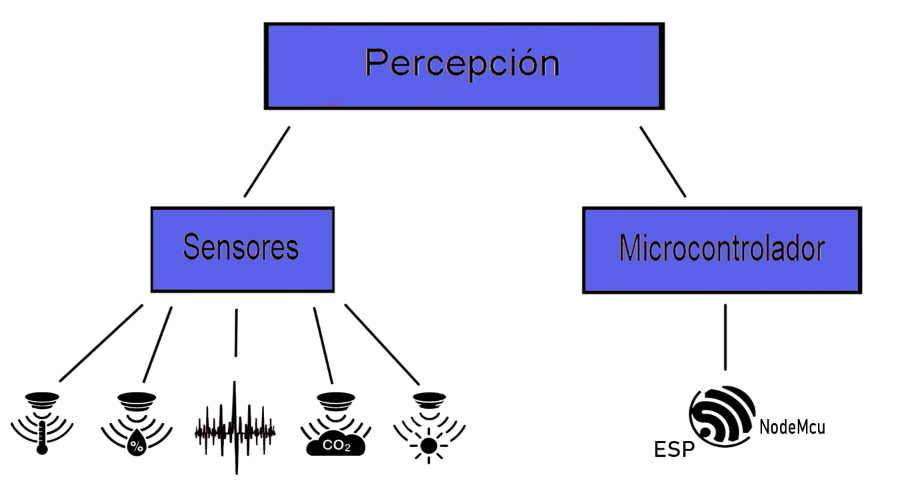
\includegraphics[width=8.5cm, height=4.5cm]{imagenes/perception_image.jpg}
        \caption{Diagrama funcional de captura de datos}
        \subcaption*{Fuente: Elaboración propia}
        \label{imag:capa_percepcion}
    \end{figure}

    \addcontentsline{toc}{subsection}{\hspace{1.3cm}1.3.2.1\hspace{5mm}Sensores} \label{subsec:sensores}
    \textbf{1.3.2.1\hspace{5mm}Sensores}
    
    Los sensores convierten estímulos físicos en señales eléctricas analógicas o digitales y según la señal se clasifican en acústicos, eléctricos, magnéticos, ópticos, térmicos y mecánicos \cite{hernandez}.
    También, se encargan de monitorear las características físicas, químicas o ambientales como: temperatura, humedad, movimiento, velocidad del viento, dirección del viento, nivel de Ph, electro conductividad, nivel de luz, entre otras \cite{lee}.

    Las señales eléctricas producidas por los sensores son proporcionales a los parámetros físicos que se monitorean y sus señales eléctricas deben ser optimizadas para el rango de entrada de los sistemas de adquisición \cite{nationalInstrument}.\\

    \textbf{Características técnicas de un sensor}
    \begin{itemize}
        \item Rango de medida: dominio en la magnitud medida en el que puede aplicarse el sensor.
        \item Precisión: es el error de medida máximo esperado.
        \item Offset o desviación de cero: valor de la variable de salida cuando la variable de entrada es nula. Si el rango de medida no llega a valores nulos de la variable de entrada, habitualmente se establece otro punto de referencia para definir el offset. (down)
        \item Linealidad o correlación lineal.
        \item Sensibilidad de un sensor: suponiendo que es de entrada a salida y la variación de la magnitud de entrada.
        \item Resolución: mínima variación de la magnitud de entrada que puede detectarse a la salida.
        \item Rapidez de respuesta: puede ser un tiempo fijo o depender de cuánto varíe la magnitud a medir. Depende de la capacidad del sistema para seguir las variaciones de la magnitud de entrada.
        \item Derivas: son otras magnitudes, aparte de la medida como magnitud de entrada, que influyen en la variable de salida. Por ejemplo, pueden ser condiciones ambientales, como la humedad, la temperatura u otras como el envejecimiento (oxidación, desgaste, etc.) del sensor.
        \item Repetitividad: error esperado al repetir varias veces la misma medida.
    \end{itemize}

    Tomado de: M.A.García y cols.\cite{caracteristicassensores}

    \newpage

    \addcontentsline{toc}{subsection}{\hspace{1.3cm}1.3.2.2\hspace{5mm}Microcontroladores}
    \textbf{1.3.2.2\hspace{5mm}Microcontroladores}

    Un microcontrolador (MCU) es un circuito integrado programable, capaz de ejecutar las órdenes grabadas en su memoria. Está compuesto de varios bloques funcionales, los cuales cumplen una tarea específica. Un microcontrolador incluye en su interior las tres principales unidades funcionales de una computadora: unidad central de procesamiento, memoria y periféricos de entrada/salida.\\

    \textbf{Características generales de los microcontroladores}

    Los microcontroladores están diseñados para reducir el costo económico y el consumo de energía de un sistema en particular. Por eso el tamaño de la unidad central de procesamiento, la cantidad de memoria y los periféricos incluidos dependerán de la aplicación.

    En este caso la aplicación que se le dará al microcontrolador será como hardware de adquisición de datos.

    Un microcontrolador típico tendrá un generador de reloj integrado y una pequeña cantidad de memoria de acceso aleatorio y/o ROM/EPROM/EEPROM/flash, con lo que para hacerlo funcionar todo lo que se necesita son unos pocos programas de control y un cristal de sincronización. Los microcontroladores disponen
    generalmente también de una gran variedad de dispositivos de entrada/salida, como convertidor analógico digital, temporizadores, UART y buses de interfaz serie especializados, como I2C y CAN.

    La memoria RAM está destinada al almacenamiento de información temporal que será utilizada por el procesador para realizar cálculos u otro tipo de operaciones lógicas. En la memoria RAM se almacenan también los registros de trabajo y configuración del procesador y los distintos periféricos del microcontrolador.

    El tipo de memoria utilizada en las memorias RAM de los microcontroladores es SRAM.
    EEPROM (Electrical Erasable Programmable Read Only Memory) y  es el sustituto natural de las memorias EPROM, la diferencia fundamental es que pueden ser borradas eléctricamente, por lo que la ventanilla de cristal de cuarzo y los encapsulados cerámicos no son necesarios.

    \newpage

    \textbf{Módulo ESP-12F}

    El módulo WiFi ESP-12F (figura \ref{imag:esp-12F}) fue desarrollado por Ai-Thinker Technology. El procesador central ESP8266 integra el micro MCU de 32 bits de potencia ultrabaja Tensilica L106 líder en la industria en un paquete pequeño con modo Lite de 16 bits, velocidad de reloj Admite 80 MHz y 160 MHz, admite RTOS e integra Wi-Fi MAC /BB/RF/PA/LNA.

    \begin{figure}[H]
        \centering
        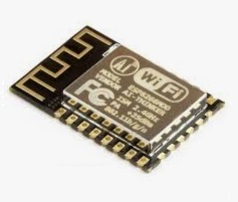
\includegraphics[width=5cm, height=5cm]{imagenes/esp-12F.jpeg}
        \caption{ESP-12F basado en ESP8266}
        \label{imag:esp-12F}
    \end{figure}

    El módulo WiFi ESP-12F es compatible con el protocolo estándar IEEE802.11 b/g/n, una pila completa de protocolos TCP/IP. Los usuarios pueden usar este módulo para agregar capacidades de red a los dispositivos existentes o para construir controladores de red separados.
    
    El ESP8266 es una solución de red Wi-Fi completa y autónoma que puede funcionar de forma independiente o como un esclavo que se ejecuta en otras MCU anfitrionas. El ESP8266 es capaz de arrancar directamente desde una memoria flash externa cuando está alimentado por una aplicación y es el único procesador de aplicaciones en el dispositivo. El caché incorporado ayuda a mejorar el rendimiento del sistema y reduce los requisitos de memoria.

    En otro caso, el ESP8266 se encarga del acceso inalámbrico a Internet. Cuando se trata de la tarea del adaptador WiFi, se puede agregar a cualquier diseño basado en un microcontrolador. La conexión es simple y fácil, solo por interfaz SPI/SDIO o puerto I2C/UART.

    Las potentes capacidades de almacenamiento y procesamiento en chip del ESP8266 le permiten integrar sensores y otros dispositivos específicos de la aplicación a través del puerto GPIO, lo que minimiza los recursos del sistema durante un desarrollo y una operación iniciales mínimos.

    Tomado de: Ai-Thinker\cite{esp12}.\\

    \textbf{Características}

    \begin{itemize}
        \item Modelo: ESP-12F
        \item Paquete: SMD22
        \item Dimensiones: 24mm x 16mm x 3mm (±0.2)mm
        \item SPI Flash: 32Mbit
        \item Interfaz de comunicación: UART, GPIO, ADC y PWM
        \item Seguridad: WEP/WPA-PSK/WPA2-PSK
        \item Modos de funcionamiento: AP, STA y STA
        \item Puertos IO: 9
        \item Puertos ADC: 1
        \item I/O voltaje tolerancia: 3.6V Max
        \item Incorpora led de prueba en el pin GPIO2
        \item Velocidad de Baudios configurable: Soporta de 300 hasta 4608000 bps, por defecto 115200 bps
        \item Antena: Incluida en el PCB
        \item Rango de frecuencia: 2412 ~ 2484 MHz
        \item Poder de transmisión: 802.11 b / g / n
            \begin{itemize}
                \item b: 16±2 dBm (@11Mbps)
                \item g: 14±2 dBm (@54Mbps)
                \item n: 13±2 dBm (@HT20, MCS7)
            \end{itemize}
        \item Voltaje de funcionamiento: desde 3.0V hasta 3.6V
        \item Voltaje de operación típico: 3.3V
        \item Corriente:
            \begin{itemize}
                \item Transmisión continua: Promedio ~2mA y Pico: 500ma
                \item Suspensión del módem: ~20mA
                \item Sueño ligero:~2mA
                \item Sueño profundo:~0.02mA
            \end{itemize}
        \item Temperatura de operación -40ºC y 85ºC
    \end{itemize}

    La principal ventaja de escoger este microcontrolador ESP-12F es por la disponibilidad de wifi sin necesidad de incorporar otros accesorios, además de las pequeñas dimensiones que posee, ideal para el desarrollo de proyectos o prototipos domóticos o de automatización en poco espacio.\\

    \addcontentsline{toc}{subsection}{\hspace{1.3cm}1.3.2.3\hspace{5mm}Nodos} \label{subsec: nodos}
    \textbf{1.3.2.3\hspace{5mm}Nodos}

    Los nodos que recopilarán los datos de cada vitrina estarán compuestos por el microcontrolador y los sensores encargados de tomar los valores medioambientales presentes teniendo en cuenta el material de las piezas expuestas dentro de cada una de las vitrinas.
    
    Estos nodos estarán ubicados también en las salas en aras de tomar datos de la habitación y relacionarlos con los obtenidos de las vitrinas.

    En base a esto, la tabla \ref{tab:correlacion_nodos} relaciona la variable a medir según la ubicación del nodo.

    \begin{table}[h]
        \centering
        \caption{Correlación de los nodos}
        \subcaption*{Fuente: Elaboración propia}
        \begin{tabular}{|l|c|l|c|}
        \hline
        \rowcolor[HTML]{9698ED} 
        \multicolumn{1}{|r|}{\cellcolor[HTML]{9698ED}Nodo} & \multicolumn{1}{r|}{\cellcolor[HTML]{9698ED}Ubicación}                      & Material objetos                                                                            & \multicolumn{1}{l|}{\cellcolor[HTML]{9698ED}Variable a medir}                                                                    \\ \hline
        1                                                  & \begin{tabular}[c]{@{}c@{}}General\\ Sala 1\end{tabular}                    & porcelana, barro, marfil                                                                    & \begin{tabular}[c]{@{}c@{}}temperatura, humedad,\\ polución, luminosidad,\\ CO2, vibraciones, salitre,\\ xilófagos\end{tabular}  \\ \hline
        2                                                  &                                                                             & bronce, barro, arcilla, piedra                                                              &                                                                                                                                  \\ \cline{1-1} \cline{3-3}
        3                                                  &                                                                             & colección numismática                                                                       &                                                                                                                                  \\ \cline{1-1} \cline{3-3}
        4                                                  &                                                                             & cerámica, madera, barro, bronce                                                             &                                                                                                                                  \\ \cline{1-1} \cline{3-3}
        5                                                  &                                                                             & \begin{tabular}[c]{@{}l@{}}madera, bronce, plata, cerámica,\\ porcelana, cuero\end{tabular} &                                                                                                                                  \\ \cline{1-1} \cline{3-3}
        6                                                  &                                                                             & barro, cerámica, plata                                                                      &                                                                                                                                  \\ \cline{1-1} \cline{3-3}
        7                                                  &                                                                             & bronce, marfil, madera                                                                      &                                                                                                                                  \\ \cline{1-1} \cline{3-3}
        8                                                  & \multirow{-7}{*}{\begin{tabular}[c]{@{}c@{}}Vitrinas\\ Sala 1\end{tabular}} & porcelana, barro policromado                                                                & \multirow{-7}{*}{\begin{tabular}[c]{@{}c@{}}temperatura, humedad,\\ luminosidad, vibraciones.\end{tabular}}                      \\ \hline
        9                                                  & \begin{tabular}[c]{@{}c@{}}General\\ Sala 2\end{tabular}                    & tela, madera                                                                                & \begin{tabular}[c]{@{}c@{}}temperatura, humedad,\\ polución, luminosidad,\\ CO2, salitre, xilófagos.\end{tabular}                \\ \hline
        10                                                 & \begin{tabular}[c]{@{}c@{}}General\\ Sala 3\end{tabular}                    & metal, plástico, tela, cuero, madera                                                        & \begin{tabular}[c]{@{}c@{}}temperatura, humedad,\\ polución, luminosidad,\\ CO2, vibraciones, salitre,\\ xilófagos.\end{tabular} \\ \hline
        11                                                 &                                                                             &                                                                                             &                                                                                                                                  \\ \cline{1-1}
        12                                                 &                                                                             &                                                                                             &                                                                                                                                  \\ \cline{1-1}
        13                                                 &                                                                             &                                                                                             &                                                                                                                                  \\ \cline{1-1}
        14                                                 & \multirow{-4}{*}{\begin{tabular}[c]{@{}c@{}}Vitrinas\\ Sala 3\end{tabular}} & \multirow{-4}{*}{cerámica (barro), piedra}                                                          & \multirow{-4}{*}{\begin{tabular}[c]{@{}c@{}}temperatura, humedad,\\ luminosidad, vibraciones.\end{tabular}}                      \\ \hline
        \end{tabular}
        \label{tab:correlacion_nodos}
    \end{table}

    Las variables ambientales a medir van estrechamente relacionadas con los sensores; estos sensores también fueron elegidos principalmente por su alto rango de mediciones ya que permiten diversos valores mínimos 
    y máximos permitiendo a su vez detectar cualquier inconveniente que pueda ser corregido mediante software sin necesidad de realizar calibraciones constantes en los laboratorios y se mantenga el sistema en invariable funcionamiento. 

    En el caso del microcontrolador lo que propone Alsuhly y cols.\cite{alsuhly} es utilizar como nodo un ESP32, un microcontrolador basado en el chip ESP8266 con bastante potencia para poder procesar la información de cada sensor de manera rápida,
    la conexion de este puede ser vía inalámbrica o por bluetooth al concentrador principal. En este caso se usará un NodeMCU, el cual es similar al ESP32 pero no contiene la interfaz bluetooth, esto permite abaratar más los costos de instalación ya que se necesitarán varios para cada vitrina de la colección.

    \subsection{Capa de Transporte}\label{subsec:capa_transporte}

    Esta es la capa responsable del traslado de la data a través de los demás componentes del sistema estableciendo la comunicación necesaria desde la toma de valores ambientales hasta su análisis y muestreo.    
    Según \cite{internetOfThingsStateOfTheArt}, la capa de transporte es la que se encarga de transportar y transmitir los datos, recopilados de la capa de percepción, hacia la cloud. Se localizan componentes de red (switch, router, Gateway, etc.), medios de comunicación y protocolos. También es responsable de aspectos de seguridad y el control de ataques.
    
    Los datos se promueven a través de protocolos MQTT, HTTP y TCP/IP.\\
    
    \addcontentsline{toc}{subsection}{\hspace{1.3cm}1.3.3.1\hspace{5mm}Protocolo MQTT}
        \textbf{1.3.3.1\hspace{5mm}Protocolo MQTT}

    MQTT son las siglas MQ Telemetry Transport, aunque en primer lugar fue conocido como Message Queing Telemetry Transport. Es un protocolo de comunicación M2M (machine-to-machine) de tipo message quere. Está basado en la pila TCP/IP como base para la comunicación. En el caso de MQTT cada conexión se mantiene abierta y se “reutiliza” en cada comunicación. Es una diferencia, por ejemplo, a una petición HTTP 1.0 donde cada transmisión se realiza a través de conexión.
    MQTT fue creado por el Dr. Andy Stanford-Clark de IBM y Arlen Nipper de Arcom (ahora Eurotech) en 1999 como un mecanismo para conectar dispositivos empleados en la industria petrolera.
    Aunque inicialmente era un formato propietario, en 2010 fue liberado y pasó a ser un estándar en 2014 según la OASIS (Organization for the Advancement of Structured Information Standards). \cite{mqtt}\\

    \addcontentsline{toc}{subsection}{\hspace{1.3cm}1.3.3.2\hspace{5mm}Protocolo HTTP}
        \textbf{1.3.3.2\hspace{5mm}Protocolo HTTP}

    HTTP de sus siglas en inglés: “Hypertext Transfer Protocol”, es el nombre de un protocolo el cual nos permite realizar una petición de datos y recursos, como pueden ser documentos HTML. Es la base de cualquier intercambio de datos en la Web, y un protocolo de estructura cliente-servidor, esto quiere decir que una petición de datos es iniciada por el elemento que recibirá los datos (el cliente), normalmente un navegador Web. Así, una página Web completa resulta de la unión de distintos sub-documentos recibidos, por ejemplo: un documento que especifique el estilo de maquetación de la página Web (CSS), el texto, las imágenes, videos, scrips, etcétera.\\


    \addcontentsline{toc}{subsection}{\hspace{1.3cm}1.3.3.3\hspace{5mm}Protocolo TCP/IP}
        \textbf{1.3.3.3\hspace{5mm}Protocolo TCP/IP}

    La definición de TCP/IP es la identificación del grupo de protocolos de red que hacen posible la transferencia de datos en redes, entre equipos informáticos e internet. Las siglas TCP/IP hacen referencia a este grupo de protocolos:

    \begin{itemize}
        \item TCP: Es el Protocolo de Control de Trasmisión que permite establecer una conexión y el intercambio de datos entre dos anfitriones. Este protocolo proporciona un transporte fiable de datos.
        \item IP o protocolo de internet, utiliza direcciones series de cuatro octetos con formato de punto decimal (por ejemplo 75.4.160.25). Este protocolo lleva los datos a otras máquinas de la red.
    \end{itemize}

    El modelo TCP/IP permite un intercambio de datos fiable dentro de una red, definiendo los pasos a seguir desde que se envían los datos (en paquetes) hasta que son recibidos. Para lograrlo utiliza un sistema de capas con jerarquías (se construye una capa a continuación de la anterior) que se comunican únicamente con su capa superior (a la que envía resultados) y su capa inferior (a la que solicita servicios) \cite{tcp/ip}.

    %Así, esta arquitectura pretende servir de referencia para la implementación de servicios basados en IoT en el área de conservación de las piezas en los museos o instituciones con vista al desarrollo de entornos inteligentes.\\

    %\section{Sistema de comunicación}\label{sec: sistemaComunicación}
    \section{Variables microclimáticas recomendadas}\label{sec:variables_microclimaticas}

    En los museos tanto universitarios como los que no poseen este tipo de característica, se requiere de un control ambiental del mismo que permita mantener el estado de conservación de los bienes patrimoniales que allí se exponen.

    En la bibliografía consultada se utiliza el concepto de conservación preventiva, la cual la define Bachman \cite{bachmann1992conservation} como un pilar básico de la gestión museológica y de la cual de ella depende el mantenimiento de las colecciones de forma adecuada, viable y sostenible en el tiempo, además de que permite la durabilidad de los elementos patrimoniales y reduce las intervenciones de los especialistas tal como lo comenta Merrit y cols. \cite{merrittPreventiveConservationHistoric2010}. Las condiciones microclimáticas más importantes a tener en cuanta según Thomson \cite{thomsonMuseumEnvironment2018} y Márquez \cite{marquezAgentesDeterioroMedioambientales2016} son la temperatura, la humedad relativa, la iluminación, las vibraciones, el CO2, la polución y el biodeterioro.

    La temperatura será tomada en grados Celcios (°C), la humedad en \%HR, el CO2 será analisado en ppm (partículas por millón), la iluminación en Luxers (Lx), la polución en micro-gramos por metros cúbicos (ug/m3) y las vibraciones en dB.

    Estos valores deben encontrarse en rangos determinados como se muestra en la siguiente tabla \ref{tab:variables_microclimaticas} según los autores Buys \& cols., Heras \& cols., Koob \& cols., Álvaro y Márquez.

    Estos valores son definidos específicamente por el tipo de clima del país, y Cuba por ser un país cálido y húmedo en algunas regiones como es la ciudad de Santiago de Cuba donde se encuentra la colección objeto de estudio de este trabajo,
    es importante realizar una valoración de los valores adecuados de estas variables ambientales por parte de los especialistas que puedan ser definidos en la propuesta y permitan mantener la colección en buen estado de conservación.
    Vale destacar que los especialistas del Centro Prat Puig han manifestado que no tienen referencia que ninguna métrica o metodología por la cual se rigan para la toma de decisiones con respecto a las variables ambientales recomendadas para la conservación de los bienes culturales de la colección.
    
    \begin{table}[H]
        \centering
        \caption{Variables microclimáticas recomendadas}
        \label{tab:variables_microclimaticas}
        \begin{tabular}{|l|l|l|l|}
        \hline
        \rowcolor[HTML]{9698ED} 
        \multicolumn{1}{|c|}{\cellcolor[HTML]{9698ED}Variables} & \multicolumn{1}{c|}{\cellcolor[HTML]{9698ED}Valores Recomendados} & \multicolumn{1}{c|}{\cellcolor[HTML]{9698ED}Material}                                                   & \multicolumn{1}{c|}{\cellcolor[HTML]{9698ED}Autor}                                                                                                                                                                                                                                    \\ \hline
                                                                & 18 - 25°C                                                         & Vidrio y Cerámicos                                                                                      & \begin{tabular}[c]{@{}l@{}}Buys y cols. \cite{buysConservationRestorationCeramics2014}\\ Heras y cols. \cite{garciaherasInnovationGestionConservacion2015}\\ Koob y cols. \cite{koobConservationRestorationGlass2004}\end{tabular} \\ \cline{2-4} 
        \multirow{-3}{*}{Temperatura}                           & 18 - 22°C                                                         & Papel, Tela, Metal y Piedra                                                                             & Álvaro \cite{recioalvaroConservacionPreventivaExposiciones2020}                                                                                                                                                                                                      \\ \cline{2-4} 
                                                                & 18 - 22°C                                                         & Madera, Pinturas.                                                                                       & \begin{tabular}[c]{@{}l@{}}Márquez \cite{marquezAgentesDeterioroMedioambientales2016}\\ Arévalo \cite{arevaloleonDegradacionArteColonial2018}\end{tabular}                                                                                          \\ \hline
                                                                & 40 - 65\%HR                                                       & Vidrio y Cerámicos                                                                                      & \begin{tabular}[c]{@{}l@{}}Buys y cols. \cite{buysConservationRestorationCeramics2014}\\ Heras y cols. \cite{garciaherasInnovationGestionConservacion2015}\\ Koob y cols. \cite{koobConservationRestorationGlass2004}\end{tabular} \\ \cline{2-4} 
        \multirow{-4}{*}{Humedad}                               & 40 - 60\%HR                                                       & \begin{tabular}[c]{@{}l@{}}Tela, Tapices, Grabados,\\ Papel.\end{tabular}                               & Arévalo \cite{arevaloleonDegradacionArteColonial2018}                                                                                                                                                                                                                \\ \cline{2-4} 
                                                                & 45 - 65\%HR                                                       & Madera, Papel, Tela                                                                                     & Márquez \cite{marquezAgentesDeterioroMedioambientales2016}                                                                                                                                                                                                           \\ \cline{2-4} 
                                                                & 30 - 50\%HR                                                       & Papel, Tela, Metal y Piedra                                                                             & Álvaro \cite{recioalvaroConservacionPreventivaExposiciones2020}                                                                                                                                                                                                      \\ \hline
        CO2                                                     & 400 - 800ppm                                                      & Papel y Tela                                                                                            & \begin{tabular}[c]{@{}l@{}}Márquez \cite{marquezAgentesDeterioroMedioambientales2016}\\ Calvo \cite{calvomanuelConservacionRestauracionPintura2002}\end{tabular}                                                                                    \\ \hline
                                                                & 300Lx                                                             & \begin{tabular}[c]{@{}l@{}}Piedra, Metal, Cerámica,\\ Vidrio.\end{tabular}                              &                                                                                                                                                                                                                                                                                       \\ \cline{2-3}
        \multirow{-4}{*}{Iluminación}                           & 150Lx                                                             & \begin{tabular}[c]{@{}l@{}}Pinturas al temple, al óleo, \\ sobre lienzo,\\ Madera, Marfil.\end{tabular} &                                                                                                                                                                                                                                                                                       \\ \cline{2-3}
                                                                & 50Lx                                                              & \begin{tabular}[c]{@{}l@{}}Papel, Tejidos, Tapices,\\ Pieles.\end{tabular}                              & \multirow{-3}{*}{Márquez \cite{marquezAgentesDeterioroMedioambientales2016}}                                                                                                                                                                                         \\ \cline{2-4} 
                                                                & 50 - 250Lx                                                        & Vidrio y Cerámicos                                                                                      & \begin{tabular}[c]{@{}l@{}}Buys y cols. \cite{buysConservationRestorationCeramics2014}\\ Heras y cols. \cite{garciaherasInnovationGestionConservacion2015}\\ Koob y cols. \cite{koobConservationRestorationGlass2004}\end{tabular} \\ \hline
        Polución                                                & 20-100 ug/m3                                                      & \begin{tabular}[c]{@{}l@{}}Pinturas, Textiles,\\ Cueros, Metales.\end{tabular}                          & Tapol \cite{tapolComoAfrontarPolucion2001}                                                                                                                                                                                                                           \\ \hline
        Vibraciones                                             & 70 - 75dB                                                         & \begin{tabular}[c]{@{}l@{}}Objetos en pedestales\\ y vitrinas\end{tabular}                              & William y cols. \cite{weiDesignVibrationDamping2011}                                                                                                                                                                                                                 \\ \hline
        \end{tabular}
    \end{table}

    \section{Condiciones que favorecen el ataque de las especies xilófagas}\label{sec:xilofagos}

    Como se analizaba en el epígrafe \ref{sec:variables_microclimaticas} el biodeterioro también constituye otro de los factores que afectan las obras de arte. Estos agentes biológicos están formados por microorganismos (bacterias) y organismos vivos como los vertebrados (aves, roedores), insectos (escarabajos, hormigas, avispas, abejas), insectos xilófagos (termitas y carcomas), moluscos (polas y gusanos de barco) crustáceos (limnorias), hongos, líquenes, algas y el propio hombre \cite{marquezAgentesDeterioroMedioambientales2016}.
    
    En el caso del control de la aparición de los xilófagos, como daño de origen biótico, no se encontró ningún sensor para medir el posible ataque, por lo que para anunciar la presencia de este tipo de anomalía se analizarán los restantes sensores y por correlación de datos será posible tenerlo en cuenta también.
    
    Por esto se realiza el análisis de las condiciones óptimas para la aparición de los mismos influyendo en la intensidad o severidad del ataque de estos insectos. Por mencionar algunos: temperatura, humedad, entre otros \cite{ripa2004termitas}. 
   
    \subsection{Temperatura}\label{subsec:xilofagos_temperatura}

    La temperatura es otro de los factores que contribuye a la aparición de los xilófagos. Según Vázquez y cols. \cite{vazquez1999avetianella}, en un experimento sobre las condiciones necesarias para la cría de plaga, parásitos y xilófagos, plantea que si estos valores de temperatura oscilan entre los 23°C y los 30°C se crean las condiciones para el surgimiento y reproducción de especies xilófagas. 

    Por otra parte Flores y Pérez \cite{floresDurabilidadNaturalDiez1987a}, en un estudio sobre los hongos xilófagos plantean que el rango de temperatura idónea para la reproducción de estos xilófagos se encuentra entre los 20°C y los 30°C, existiendo también el caso de que aún con 38°C exista la posibilidad de reproducción en algunas especies, así como Avalos Díaz y cols. \cite{avalosdiazInfluenciaDosHongos2020} que en una de sus publicaciones se define que la temperatura idónea para el surgimiento de colonias xilófagas es de 27°C +- 1.
   
    \subsection{Humedad}\label{subsec:xilofagos_humedad}

    El contenido de agua de la madera constituye uno de los factores más importantes que favorecen el ataque de las especies xilófagas. Maderas con un contenido de humedad sobre el 15\% favorece las infestaciones de coleópteros xilófagos, acortando significativamente sus ciclos de vida lo que aumenta sus poblaciones y la posibilidad de reinfestaciones \cite{ripa2004termitas}, esto relacionado a que la acumulación de humedad se acentúa en construcciones con escasa ventilación, la que se debe incrementar en espacios interiores.

    Según Araquistain y col. \cite{monitoringMoisture} y Rodríguez y col. \cite{rodriguezcodigo}, el porcentaje de humedad óptimo para que crezcan los xilófagos está entre el 25 y el 55\% mientras que Kisternaya \cite{woodPreservation} plantea que, el rango de humedad idónea puede estar entre el 35 y el 50\%. Tomando estos porcentajes de humedad idóneos para la aparición de los xilófagos, se establece como valor máximo de humedad un 20\%.

    
    \section{Principales afectaciones}\label{sec:principales_afectaciones}

    \textbf{¿Qué ocurre si los valores microclimáticos no se encuentran en el rango de lo recomendado?}

    A continuación se analiza por variable microclimática la afectación que trae consigo esta variación según autores.

    \textbf{Temperatura}

    Según Márquez \cite{marquezAgentesDeterioroMedioambientales2016} una temperatura elevada favorece la velocidad de los procesos químicos, con esto un aumento de 10°C duplica la velocidad de los procesos reproductores del moho y favorece  el desarrollo del biodeterioro en presencia de altas HR (plagas), además de que provoca la evaporación del agua de composición de los materiales dando lugar a la sequedad y deshidratación de los mismos, que originan su degradación.

    Mientras que Álvaro \cite{recioalvaroConservacionPreventivaExposiciones2020} plantea que una temperatura contraindicada (demasiado alta, demasiado baja o fluctuaciones) provoca alteraciones de los colores y desintegración progresiva de los materiales orgánicos, especialmente si son químicamente inestables como el papel ácido, fotografías en colores, entre otros, así como el agrietamiento de pinturas y otros polímeros a causa de la frialdad.

    En el caso de Gómez \cite{gomezcarreteroEfectosAcidoNitrico2015a} plantea que la temperatura es un factor de envejecimiento del óleo. Actúa de modo semejante y en combinación con la luz, y produce cambios de humedad relativa al aumentar o disminuir la temperatura ambiental.

    \textbf{Humedad}

    La humedad excesiva constante superior al 75\% puede provocar: debilitación de adhesivos, pudrimiento de colas, aumento del tamaño de los materiales (madera, papel, tela, etc.), manchas (papel, tela, vitela, etc.), corrimiento de tintas, enmohecimiento de cueros, aumento de la corrosión de los diferentes metales, adherencia de hojas de papel, ablandamiento de materias, aparición de sales, opacidad de vidrios, entre otras. Al igual que la sequedad excesiva constante inferior al 35\% puede producir: fragilidad y desecación de los componentes de las obras, deterioro en maderas y marqueterías por contracción, tensión de las telas, reducción dimensional de materiales, entre otras.\cite{marquezAgentesDeterioroMedioambientales2016}

    Del mismo modo que el cambio brusco en estos niveles de humedad puede provocar:
    \begin{itemize}
        \item Alteración de los colores y desintegración gradual de materiales orgánicos, especialmente de aquellos químicamente inestables como el papel ácido.
        \item Aparición de moho en materiales orgánicos e inorgánicos; corrosión en metales y encogimiento en textiles.
        \item Procesos de hidratación o deshidratación de ciertos minerales y corrosión de los metales que contengan sales.
        \item Procesos de contracción, dilatación, compresión y agrietamiento de los materiales orgánicos en función del efecto de las fuerzas.
    \end{itemize}
    Tomado de Álvaro \cite{recioalvaroConservacionPreventivaExposiciones2020}.\vspace{0.5cm}

    Así mismo Gómez \cite{gomezcarreteroEfectosAcidoNitrico2015a} plantea que si la humedad relativa se incrementa y el agua se condensa en la superficie de los objetos, los materiales sensibles a la humedad aumentan de volumen. Entre estos materiales se hallan los tejidos, el papel y la madera. Cuando la humedad relativa desciende, estos objetos se contraen. Los fenómenos de contracción y dilatación producen grietas y deformaciones.

    \textbf{CO2}

    Según Calvo \cite{calvomanuelConservacionRestauracionPintura2002} el CO2 combinado con agua produce el ácido carbónico, que afecta a los materiales orgánicos y produce corrosión en los materiales pétreos y el vidrio.

    Las reacciones de fotooxidación son inevitables y hacen que las capas pictóricas pierdan sus propiedades.\cite{gomezcarreteroEfectosAcidoNitrico2015a}

    \textbf{Iluminación}

    La iluminación es un importante factor de deterioro ya que tanto la luz visible como las radiaciones UV activan la formación de radicales libres en los enlaces múltiples de las cadenas insaturadas de los aceites secantes que aglutinan la pintura al óleo.\cite{gomezcarreteroEfectosAcidoNitrico2015a}

    Según Márquez \cite{marquezAgentesDeterioroMedioambientales2016} en el papel la luz provoca decoloración, cambio de color (tono amarillo) y rotura de enlaces químicos, dando lugar a su envejecimiento prematuro, que lo vuelve quebradizo, produciendo el debilitamiento de su estructura, también las pinturas a la acuarela se ven afectadas por la decoloración de la materia pictórica y los efectos de la luz sobre el papel y en los tejidos, la luz produce rotura y debilitamiento de la materia por fragmentación de sus enlaces químicos.

    \textbf{Polución}

    En el caso de los efectos negativos de la polución sobre los metales, y más concretamente el plomo, la plata y el bronce, provocando pérdida de brillo, picaduras, manchas, cambios de color, eflorescencias, entre otras.
    De la misma manera que las pinturas y los papeles amarillean y se debilitan, los textiles pierden resistencia mecánica, los colorantes cambian de tonalidad, las gomas se cuartean y los cueros cobran un aspecto polvoriento.\cite{tapolComoAfrontarPolucion2001}

    \textbf{Vibraciones}

    Según Sánchez \cite{sanchezPinturaSobreTabla2015} las vibraciones producen efectos acumulativos que traen consigo la degeneración, el envejecimiento y fatiga de los componentes, esto uniéndose a la edad en el caso de las pinturas.

    Por otra parte, Ortiz \cite{ortizRestauracionObrasArte2012} plantea que las vibraciones bruscas generan fisuras o la aparición de pequeñas grietas que dañan la capa pictórica de los cuadros llegando a pulverizarse, al igual que el daño en los soportes de los mismos.

    \textbf{Xilófagos}

    Como parte de los daños ocasionados por las especies xilófagas se encuentran los planteados por Ortiz \cite{ortizRestauracionObrasArte2012}, el cual plantea que estos afectan directamente la estructura de los lienzos debilitando el entramado de los hilos que componen la tela trayendo consigo el deterioro total casi irreparable en caso de no tratarse a tiempo.

    Por otro lado Romero y cols. \cite{ferrerasromeroVirgenConNino2011} afirma que el ataque de los insectos xilófagos trae consigo daños al soporte lignario de las obras de arte ocasionando daños de diferente índole, desde pequeños orificios de salida de los xilófagos hasta zonas puntuales donde la madera se convierte en un material completamente disgregado.

    \newpage

    \addcontentsline{toc}{section}{Conclusiones}
    \textbf{\large Conclusiones parciales}

    Como parte del análisis desarrollado en este capítulo:
    
    \begin{itemize}
        \item Se habló de la variedad de aplicaciones del Internet de las Cosas y de su relación con la conservación del patrimonio cultural. La descripción de las arquitecturas del IoT brindó la posibilidad de proponer la arquitectura del sistema que se desea implementar.
        \item Como parte del análisis de este sistema se explicó el concepto de sensor, de aquí se concluye que estos serán la unidad básica de adquisición de la información para nuestra arquitectura.
        \item Se explicó el concepto de microcontrolador, fundamentando que se selecciona ESP-12F sobre las demás plataformas por las características expuestas anteriormente.
        \item Se establecieron valores mínimos y máximos a modo de evitar la aparición del especies xilófagas en la colección objeto de estudio.
        \item Se analizaron las principales formas en las que se manifiestan los daños en distintos materiales ocasionados por valores microclimáticos fuera del rango de lo recomendado. 
    \end{itemize}